
%(BEGIN_QUESTION)
% Copyright 2013, Tony R. Kuphaldt, released under the Creative Commons Attribution License (v 1.0)
% This means you may do almost anything with this work of mine, so long as you give me proper credit

Draw connecting wires that will create a {\it series-parallel} circuit, such that the voltage dropped across $R_1$ will be twice as much as the voltage dropped across $R_2$ or $R_3$.  Make sure each resistor drops voltage in the polarity shown by the (+) and ($-$) symbols:

$$\includegraphics[width=15.5cm]{i03561x01.eps}$$

\begin{itemize}
\item{} Supposing the battery has a voltage of 12 volts, and all resistors are 1 k$\Omega$ in resistance value, calculate the voltage dropped by each resistor.
\item{} Supposing the battery has a voltage of 12 volts, and all resistors are 1 k$\Omega$ in resistance value, calculate the current passing through each resistor as well as the current passing through the battery.
\end{itemize}

\underbar{file i03561}
%(END_QUESTION)





%(BEGIN_ANSWER)

Bear in mind that this is not the {\it only} possible circuit solution:

$$\includegraphics[width=15.5cm]{i03561x02.eps}$$

Challenge yourself by designing a different circuit to meet the same criteria! 

%(END_ANSWER)





%(BEGIN_NOTES)


%INDEX% Pictorial circuit review (series-parallel resistor circuit)

%(END_NOTES)


